\chapter{Secure (signed) Electronic Documents}

Let's start, as always with some definitions.
\begin{boxH}
  An \textbf{electronic document} is any \textbf{electronic
  representation} of a \textbf{document}, while a \textbf{digital
  document} is a \textbf{digital representation} of a document.
\end{boxH}

Secure electronic documents must satisfy the following properties:
\begin{itemize}
    \item \textbf{Security:} Ensure data integrity and authenticity
      using a digital signature.
    \item \textbf{Readability:} Use an open format for content and
      signature interpretation.
    \item \textbf{Long-term Archival:} Ensure readability and
      verifiability over decades.
\end{itemize}

\section{Formats of Signed Documents}
Signed documents can take different formats:
\begin{itemize}
    \item \textbf{Enveloped Signature:} The signature is embedded
      within the document in a specific location (e.g., PDF).
    \item \textbf{Enveloping Signature(another case):} The document is
      embedded within the signature structure (e.g., PKCS\#7).
    \item \textbf{Detached Signature:} The signature is separate from
      the document (e.g., PKCS\#7). In this case the correlation
      between the signature of the document(for instance, using a
      pointer).
\end{itemize}

\begin{figure}[H]
  \centering
  \includegraphics[width=0.5\textwidth]{img/signed documents
  format.png}
  \caption{Different formats of signed documents.}
\end{figure}

\section{Multiple signatures}
In most case, multiple signatures are needed, for example in an office
there is typically a specific document workflow: an purchase order 
may need to be validated and approved by different people, each of 
which will sign the document.

In those scenarios, the signatures can be either parallel or
sequential. In case of independent signature, each signature is applied
to the original document, while in case of sequential signature, each 
signature is applied to the previous signed document.
\begin{figure}[H]
  \centering
  \begin{subfigure}[b]{0.45\textwidth}
    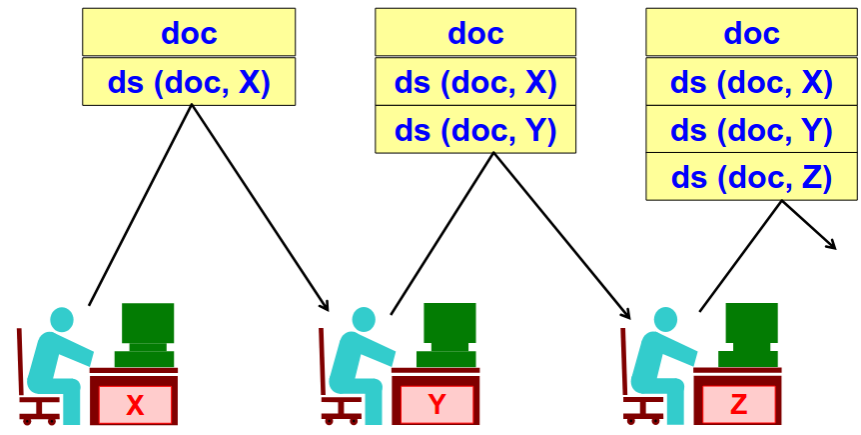
\includegraphics[width=\textwidth]{img/paralledl signatures.png}
    \caption{Parallel signatures in a single document.}
  \end{subfigure}
  \hfill
  \begin{subfigure}[b]{0.45\textwidth}
    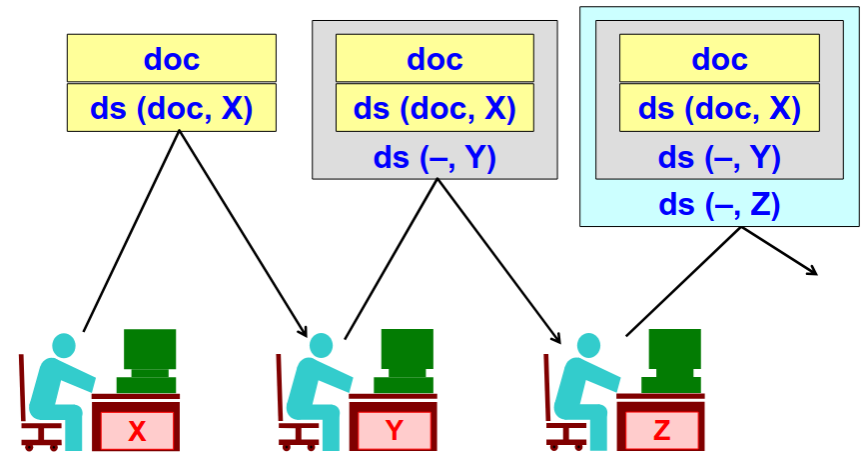
\includegraphics[width=\textwidth]{img/sequential signatures.png}
    \caption{Sequential signatures in a single document.}
  \end{subfigure}
\end{figure}

\section{Digital Signatures in PDF Files}

When a PDF needs to be signed, it is at first converted in a byte
stream, while also reserving a specific place for the signature.

The data to be signed is identified by two intervals:
\begin{verbatim}
/ByteRange[ offset1, length1, offset2, length2 ]
\end{verbatim}

Then, a digest of the data(signature excluded) is compute, for example
using sha-256, which is afterward encrypted with the signed private
key, via RSA-2048 for instance.

The signature value is encoded as a PKCS\#7 detached signature, and
the hex encoded signature value is inserted in the reserved space,
along with the necessary padding(made up of zeroes).

Logically, the signature is detached from the document, but in a pdf
it is actually embedded in the document.


\begin{figure}[H]
  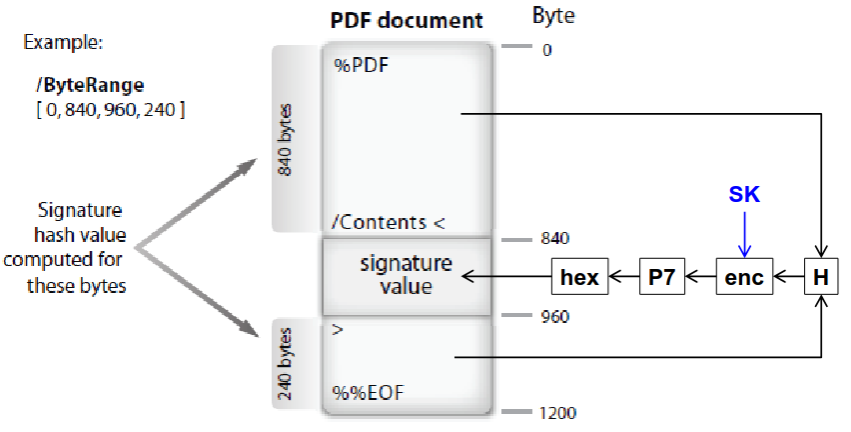
\includegraphics[width=.6\textwidth]{img/pdf digital signature.png}
  \caption{Digital signature in a pdf file}
  \label{fig:pdf digital signature}
\end{figure}


\section{Adobe Acrobat Signature Formats}
Adobe Acrobat supports the following signature formats:
\begin{itemize}
    \item \texttt{adbe.pkcs7.detached} (default).
    \item \texttt{adbe.pkcs7.sha1}.
    \item \texttt{adbe.x509.rsa.sha1}.
    \item \texttt{ETSI.CAdES.detached} (since Acrobat 10.x).
\end{itemize}
but also supports custom signature handlers, while retaining the same
structural format.

\subsection{Adobe Acrobat signature algorithms}
Adobe Acrobat provides support for various signature algorithms, which
evolve based on the Acrobat and PDF version. The details of supported
message digest algorithms and encryption or signature methods are as
follows:

\begin{itemize}
    \item \textbf{4.x–5.x} / PDF 1.3: MD5, SHA1
    \item \textbf{6.x} / PDF 1.3: MD5, SHA1
    \item \textbf{7.x} / PDF 1.6: MD5, SHA1, SHA256
    \item \textbf{8.x–9.0} / PDF 1.7: MD5, SHA1, SHA256, SHA384,
      SHA512, RIPEMD160
    \item \textbf{9.1–9.x} / PDF 1.7: MD5, SHA1, SHA256, SHA384,
      SHA512, RIPEMD160
    \item \textbf{10.x and later} / PDF 1.7: MD5, SHA1, SHA256,
      SHA384, SHA512, RIPEMD160
\end{itemize}

\subsection*{Encryption or Signature Algorithms}
\begin{itemize}
    \item \textbf{4.x–5.x} / PDF 1.3: RSA up to 1024-bit
    \item \textbf{6.x} / PDF 1.5: RSA up to 4096-bit
    \item \textbf{7.x} / PDF 1.6: RSA and DSA up to 4096-bit
    \item \textbf{8.x–10.x} / PDF 1.7: RSA and DSA up to 4096-bit
    \item \textbf{11.x and later} / PDF 1.7:
    \begin{itemize}
        \item RSA and DSA up to 4096-bit
        \item ECDSA P256-SHA256, P384-SHA384, or P512-SHA512
          (available only with \texttt{adbe.pkcs7.detached} and
          \texttt{ETSI.CAdES.detached})
    \end{itemize}
\end{itemize}

DSA supports only SHA1 (by design) and can only be used in
\texttt{adbe.pkcs7.detached}.


\begin{wrapfigure}{r}{0.4\textwidth}
  \centering
  \includegraphics[width=0.4\textwidth]{img/adobe multiple
  signatures.png}

  % \caption{CT System Configuration}
\end{wrapfigure}

\section{Electronic Signature (ES) and Advanced Electronic Signature
(AES)}
An ES is defined as:
\begin{boxH}
    Data in electronic form, attached to or logically associated with
    other electronic data, serving as a method of authentication.
\end{boxH}

On the other hand, an AES satisfies additional requirements:
\begin{itemize}
    \item Uniquely linked to the signatory.
    \item Capable of identifying the signatory.
    \item Created under the signatory's sole control.
    \item Detects any subsequent changes to the signed data.
\end{itemize}

\section{Qualified Certificate (QC)}


\subsection{Qualified Electronic Signature (QES)}
A QES is:
\begin{itemize}
    \item An AES based on a Qualified Certificate (QC).
    \item Created by a secure signature creation device.
    \item Legally equivalent to a handwritten signature.
\end{itemize}

\begin{figure}[H]
  \centering
  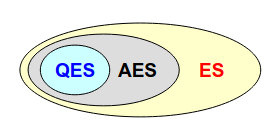
\includegraphics[width=0.4\textwidth]{img/es-aes-qus.png}
  \caption{Electronic Signature (ES), Advanced Electronic Signature
  (AES), and Qualified Electronic Signature (QES).}
\end{figure}

\section{Legal effects}
Member States shall ensure that an electronic signature is not denied
legal effectiveness and admissibility as evidence in legal proceedings
solely on the grounds that it is:
\begin{itemize}
  \item in electronic form, or
  \item not based upon a qualified certificate, or
  \item not based upon a qualified certificate issued by an accredited
    certification-service-provider, or
  \item not created by a secure signature-creation device
\end{itemize}


\chapter{Standards for Electronic Signatures}

\section{ETSI Standards}
ETSI standards for electronic signatures include:
\begin{itemize}
    \item \textbf{CAdES:} CMS Advanced Electronic Signatures.
    \item \textbf{XAdES:} XML Advanced Electronic Signatures.
    \item \textbf{PAdES:} PDF Advanced Electronic Signatures.
    \item \textbf{ASiC:} Associated Signature Containers for detached signatures.
\end{itemize}

\section{CAdES Formats}
\begin{itemize}
    \item \textbf{ES-C:} Includes complete certificate and revocation references.
    \item \textbf{ES-T:} Adds a timestamp over the digital signature.
    \item \textbf{ES-X:} Extends ES-C with additional timestamps for enhanced validation.
\end{itemize}

\chapter{Trust and Validation}

\section{Trust Service Status List (TSL)}
TSL is a signed list containing Trust-Service Providers (TSPs) and their services. It tracks the state (e.g., supervised, suspended) and history of each TSP.

\section{WYSIWYS}
\textbf{What You See Is What You Sign (WYSIWYS)} ensures that the displayed document content is what is actually signed. It is a legal requirement in some jurisdictions, such as Austria.

\section{Final Warnings}
Be cautious of software bugs. For example, an older version of the Postecom signature tool accepted invalid root certificates embedded within the PKCS\#7 signature.

\end{document}
